% ****** Start of file aipsamp.tex ******
%
%   This file is part of the AIP files in the AIP distribution for REVTeX 4.
%   Version 4.1 of REVTeX, October 2009
%
%   Copyright (c) 2009 American Institute of Physics.
%
%   See the AIP README file for restrictions and more information.
%
% TeX'ing this file requires that you have AMS-LaTeX 2.0 installed
% as well as the rest of the prerequisites for REVTeX 4.1
%
% It also requires running BibTeX. The commands are as follows:
%
%  1)  latex  aipsamp
%  2)  bibtex aipsamp
%  3)  latex  aipsamp
%  4)  latex  aipsamp
%
% Use this file as a source of example code for your aip document.
% Use the file aiptemplate.tex as a template for your document.
\documentclass[%
 aps,
 %jmp,%
 %prb,
 prl,
 amsmath,amssymb,
 %preprint,%
 %superscriptaddress,
 reprint,%
 %floatfix,
%author-year,%
%author-numerical,%
]{revtex4-1}
%]{article}

\usepackage{graphicx}% Include figure files
\usepackage{dcolumn}% Align table columns on decimal point
\usepackage{bm}% bold math
%\usepackage[mathlines]{lineno}% Enable numbering of text and display math
%\linenumbers\relax % Commence numbering lines

% Alter some LaTeX defaults for better treatment of figures:
    % See p.105 of "TeX Unbound" for suggested values.
    % See pp. 199-200 of Lamport's "LaTeX" book for details.
    %   General parameters, for ALL pages:
    \renewcommand{\topfraction}{0.9}    % max fraction of floats at top
    \renewcommand{\bottomfraction}{0.8}    % max fraction of floats at bottom
    %   Parameters for TEXT pages (not float pages):
    \setcounter{topnumber}{2}
    \setcounter{bottomnumber}{2}
    \setcounter{totalnumber}{4}     % 2 may work better
    \setcounter{dbltopnumber}{2}    % for 2-column pages
    \renewcommand{\dbltopfraction}{0.9}    % fit big float above 2-col. text
    \renewcommand{\textfraction}{0.07}    % allow minimal text w. figs
    %   Parameters for FLOAT pages (not text pages):
    \renewcommand{\floatpagefraction}{0.7}    % require fuller float pages
    % N.B.: floatpagefraction MUST be less than topfraction !!
    \renewcommand{\dblfloatpagefraction}{0.7}    % require fuller float pages
    % remember to use [htp] or [htpb] for placement
    \setlength{\abovecaptionskip}{0pt}
    \setlength{\belowcaptionskip}{0pt}
    \setlength{\parskip}{0pt}
    \setlength{\textfloatsep}{1pt} 

\begin{document}
%\title{Reduction of turbulent fluctuations and crossphase through driven sheared flow on the Large Plasma Device}
\title{Observation of improved and degraded confinement with driven flow on the LAPD}
\author{D.A. Schaffner}
\author{T.A Carter}
\author{G.D. Rossi}
\author{D.S. Guice}
\author{J. Maggs}
\author{S. Vincena}
\author{B. Friedman}
	\affiliation{Department of Physics and Astronomy, University
          of California, Los Angeles.}%Lines break automatically or can be forced with \\

\date{\today}% It is always \today, today,
             %  but any date may be explicitly specified

\begin{abstract}
Continuous control over the azimuthal flow and flow shear in the edge region of the Large Plasma Device (LAPD) has been acheived using a biasable limiter allowing a detailed study of the effect of flow shear on turbulence and transport in LAPD, extending previous work~\cite{carter09}. LAPD rotates spontaneously in the ion diamagnetic direction (IDD); positive limiter bias allows this spontaneousflow to be reduced, minimized (producing a near-zero flow and flow
shear state), and reversed to strong flow in the electron diamagnetic direction (EDD). In the minimum flow/shear state, confinement is degraded relative to the spontaneously flowing LAPD edge while edge gradient scale length, flucutation amplitude and particle flux increas. With shearing near decorrelation rate, flux and isat fluctuations decrease by 50\%. At five times decorrelation, reduction is 80\%. The variation is insensitive to flow direction but show differences in scaling by frequency range.The variations of flux, density fluctuation amplitude, crossphase and radial correlation length with shearing rate are compared to power laws fits.
\end{abstract}

\maketitle
%\section{Introduction}  No need for section titles in PRL, save space

%% Need to start with discussion of H-mode, role of flow.  Cite BDT, recent reviews of flow-shear interaction (Terry, Diamond, Tynan).  Move immediately to set up why this study is unique

	The effect of flow and flow shear on plasma turbulence has long been studied as a mechanism for turbulence reduction and increased particle confinement in both tokamaks and linear machines.  The most dramatic observed effect of cross-field flow is the creation of a higher confinement state, called an H-mode, which has been first observed on ASDEX\cite{wagner82} and later on other tokamaks such as the Continuous Current Tokamak (CCT)\cite{taylor89,tynan92} and DII-D\cite{groebner90,moyer95}. While some plasma machines rely on a spontaneous flow for study (CSDX ref), other machines including TEXTOR\cite{boedo00} and LAPD\cite{maggs07,carter09} have developed external biasing mechanisms to produce radial electric fields which can drive controllable azimuthal flow by $E \times B$ drift\cite{weynants93}.

Theoretical investigation into the nature of effect of sheared flow has focused mainly on its influence on turbulent fluctuations \cite{biglari90} and on the crossphase between electric field and any advected quantity, such as density in the case of particle flux \cite{ware96,terry01}. Fluctuation reduction by shear is thought to come by the reduction in radial correlation length---shearing of turbulent eddies---while the effect of crossphase has to do with the fact that turbulent particle flux relies on the phasing of outward or inward ExB flows with increases in density. The simplest mode non-specific models for the effect of shearing on turbulent fluctuations predict a power law decrease\cite{biglari90}, while crossphase can have an even stronger scaling\cite{terry01}.

The experiment in this letter is an extension of previous biasing experiments on LAPD. In one, an inward pointing electric field produced by chamber biasing demonstrated that increased flow shear resulted in turbulent modification and increased particle confinement\cite{carter09}. However, penetration of the electric field was low until high biases resulting in sudden transition from background states to confined states. In another experiment, it was shown that a small biased annulus could produce sheared flows within the main column of the plasma\cite{zhou12}. A new biasing mechanism has allowed for a smooth transition from a low flow shear state in the IDD---LAPD's natural state---to zero shear state, to a high shear state in the EDD. With this smooth control of flow shear, we can carefully observe the effect of shear on turbulent fluctuations, particle flux, and gradient length scale to a level of detail that allows for comparison to theory prediction.

In this letter, we report on the observation of a degraded and enhanced confinement state as a function driven sheared flows ranging from no shear to up to five times a no-shear turbulent decorrelation rate. This confinement occurs regardless of flow or flow shear direction. We have shown that this variation in confinement correlates with particle flux levels. Moreover, we can show that radial correlation length, particle flux, crossphase, density fluctuations all decrease with shearing rate and that substantial decreases begin with rates as small as one-half the turbulent decorrelation rate. We observe differing characteristics depending on which frequency regime in examined. Namely, we see that suppression of flux at frequencies less than 10kHz are dominated by decreases in density fluctuations while flux suppression at greater than 10kHz is dominated by crossphase and coherency decreases. We note that electric field fluctuations appear to be minamally affected by shearing changes. Lastly, we can fit the various quantities to a power-law decay for comparison to theory predictions \cite{biglari90}.

The Large Plasma Device \cite{gek91} (LAPD) is a 20m by 1m cylindrical linear device with a 54cm wide barium-oxide coated nickel cathode pulsed at 1Hz to produce a 45eV electron beam which ionizes the helium gas in the chamber. A column long plasma of density about $5 \times 10^{12}$ cm$^{-3}$ and temperature of 5eV is produced. The field for this experiment was set to 1000G. To produce the bias, four quarter annulus aluminum plates are inserted half a meter axially beyond the cathode creating a flat boundary condition radially from the chamber wall to the opening of a 26cm aperture. A pulse power circuit connected to a capacitor bank supplies a 5ms bias during the 15ms plasma discharge ranging from floating potential to 230V referenced from the cathode. Measurements of saturated current and floating potential are taken with a 9-tip flush surface tantalum probe while temperature and plasma potential is taken by swept Langmuir probe.

Azimuthal flow and flow shear are controlled by adjusting the voltage on the limiter plates. When voltages on the limiter on are less than the voltage of the anode, an overall azimuthal flow occurs in the IDD as shown in
Fig.~\ref{fig:velocity_flowshear}
with velocities peaking just outside the limiter edge. When the voltage on the limiter is brought near anode potential, flow and flow shear zero out. Voltages above anode produce electron diamagnetic direction flows peaked at the limiter edge. The voltage on the power supply cannot be set below the floating potential as the plasma tends to charge the capacitor banks.

Measurements of ion saturated current and particle flux are taken for each bias flow state. A set of radial values are averaged over a range from 27 to 31cm in a region where such averaged flow and flow shear scale approximately linearly with limiter bias as in 
Fig.~\ref{fig:velocity_flowshear}%
and are outside the limiter edge to avoid any possible effects from primary electrons. Maxing out at about 125kHz, we can achieve a shearing rate of approimately five times the natural turbulent decorrelation rate. The no flow, no shear regime allows us to directly measure a turbulent decorrelation rate. An autocorrelation time of about 36us is calculated by taking the full width at half max of a Hilbert transform of the isat autocorrelation function at the no flow/shear bias yielding a decorrelation rate of $\Delta \omega_{t} = $ 28kHz.

Calculated quantites are used to characterize flux and length scale. Density gradient length scale is calculated by $L_{n} = \lvert \nabla \ln n \rvert ^{-1}$ while particle flux, $\Gamma_{p} = \langle \tilde{n} \tilde{v_{r}} \rangle = \langle \tilde{n} \tilde{E_{\theta}} \rangle /B$, can be calculated spectrally as\cite{powers74}, 
\begin{equation}
\Gamma_{p} = \frac{2}{B} \int^{\infty}_{0} \lvert n(\omega) \rvert \lvert E_{\theta}(\omega) \rvert \gamma_{n,E_{\theta}}(\omega) \cos [\phi_{n,E_{\theta}}(\omega)] d\omega
\label{eq:fluxint}
\end{equation}
which also allows us to directly determine the contributions of turublent fluctuations, crossphase and coherency to the particle flux.

The first clear result shown in Fig.~\ref{fig:densgrad} is a change in particle confinement level as bias is varied, as indicated by a change in the gradient scale length of the density radial profiles. The average density gradient scale length begins at 9cm with no bias, but at the point of minimum shearing rate, the density gradient levels out, reaching a scale length peak of about 15cm. As bias and shearing 
\begin{figure}
\begin{center}
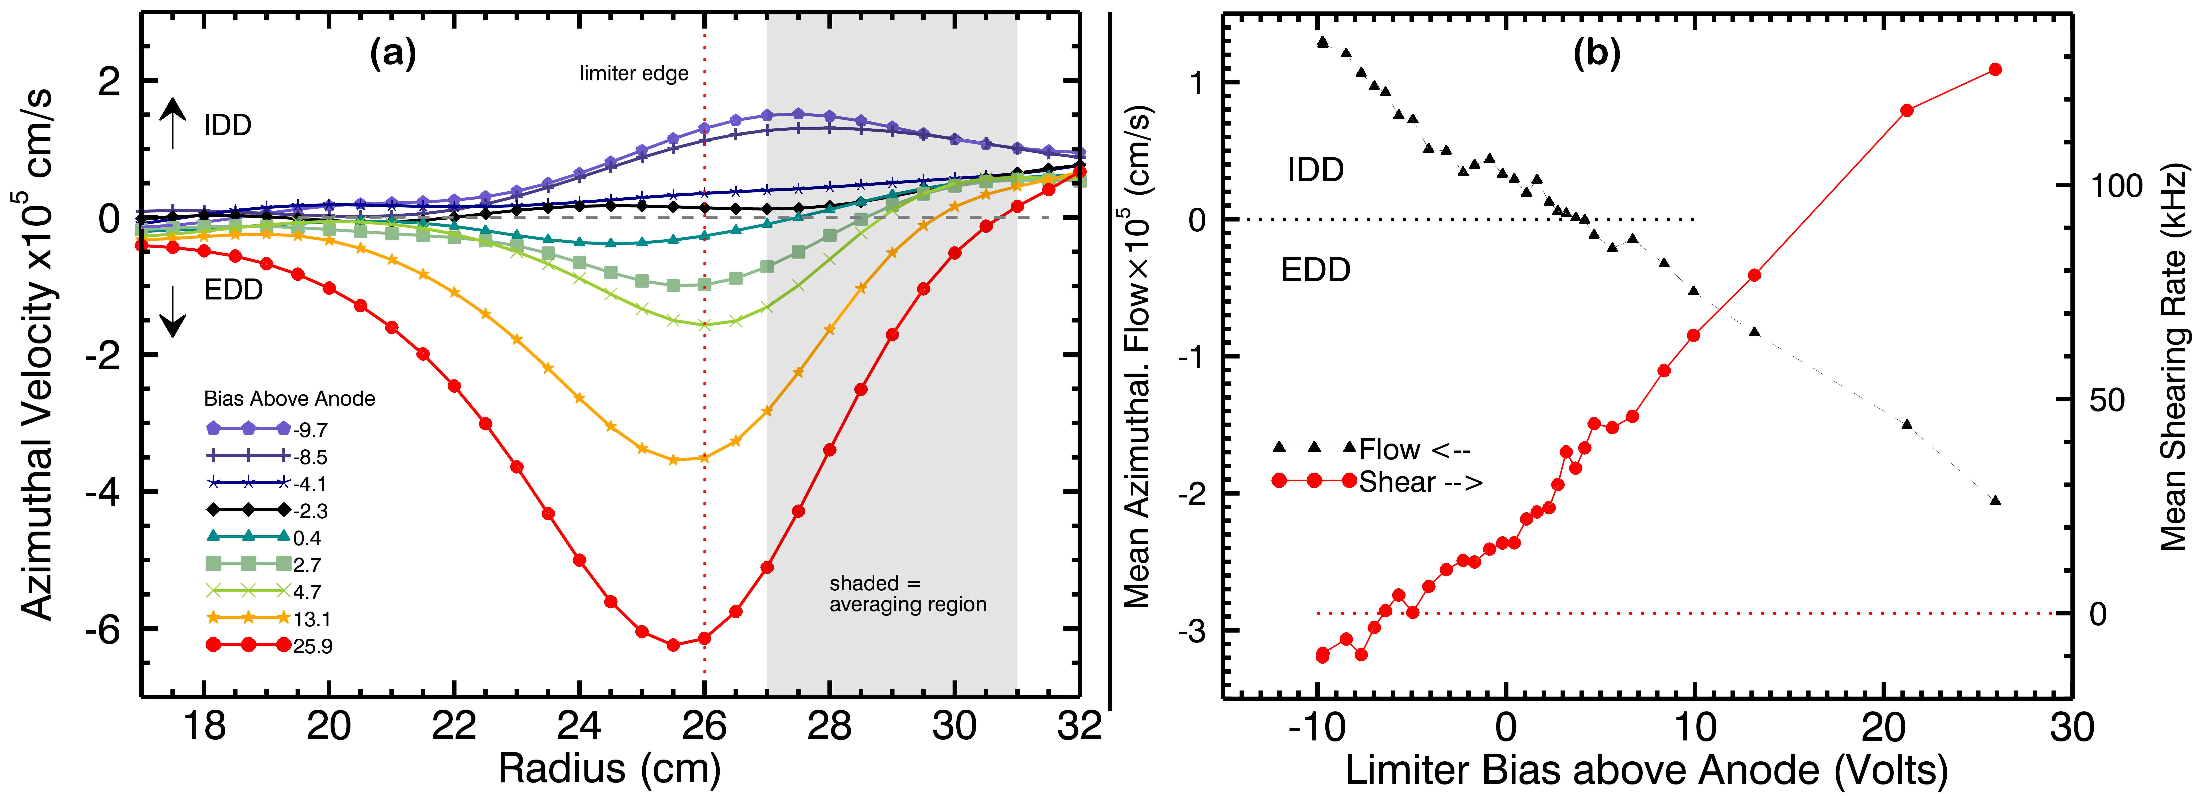
\includegraphics[width=8.5cm]{velocity_flowshear.pdf}% Here is how to import EPS art
\caption{\label{fig:velocity_flowshear} (a) Velocity profiles using plasma potential from swept measurements. (b) Nearly linear scaling of flow (black) and shearing (red) versus limiter bias.}
\end{center}
\end{figure}
continue to increase, the density gradient steepens again. Higher voltage causes the density gradient to steepen further reaching a saturated value of about 5cm. The initial scale length value and saturated values are consistent with previous biasing experiments done on the LAPD\cite{carter09}, but rather than see a density gradient degradation, a sharp threshold is observed. It is likely the new biasing setup allows this transition to be observed. It was spectulaed in the previous experiment that a threshold was observed not because of an inherent dependence on a shear value, but because of penetration of cross-field current---and thus flow---from the chamber edge to the plasma source. By placing the limiters---the source of biasing current---closer to the cathode edge---the electron source, we can establish cross-field currents at lower shear values than before.

\begin{figure}
\begin{center}
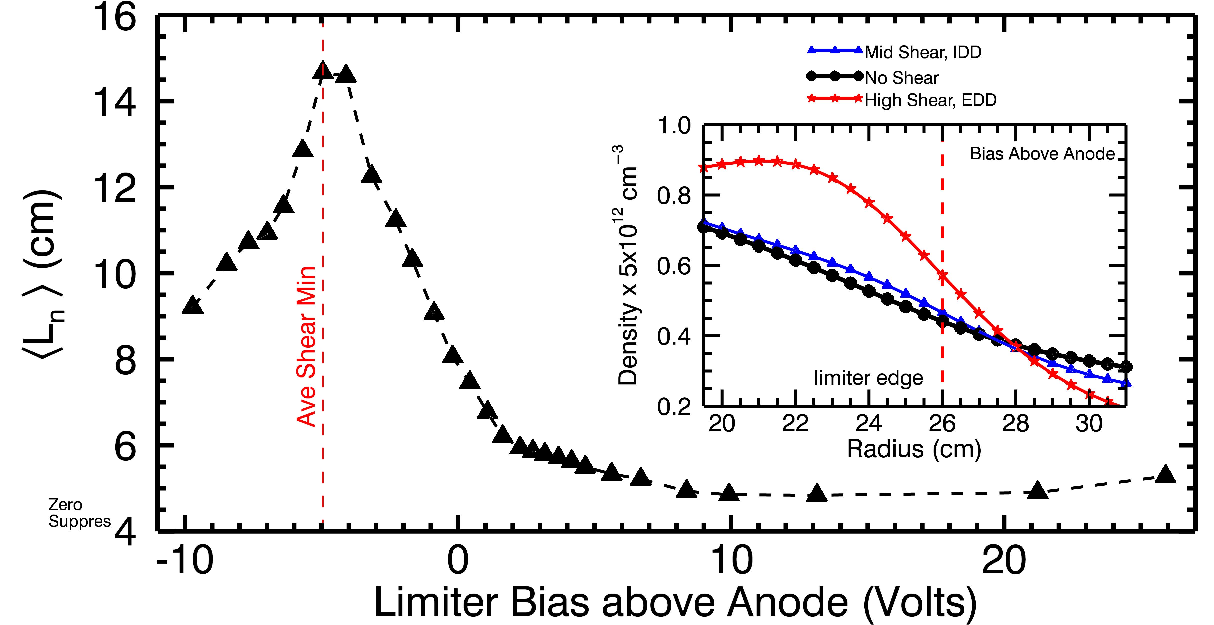
\includegraphics[width=8.5cm]{densgrad.pdf}% Here is how to import EPS art
\caption{\label{fig:densgrad} Density gradient length scale versus limiter bias. Inset shows density profile relaxing then steepening again with bias.}
\end{center}
\end{figure}

Also note the symmetry of the gradient scale length curve about the shear minimum. This is an indication that both IDD or EDD flow and shearing direction can produce a steepened density gradient. This is clearly seen in
Fig.~\ref{fig:shearandgrad}

\begin{figure}
\begin{center}
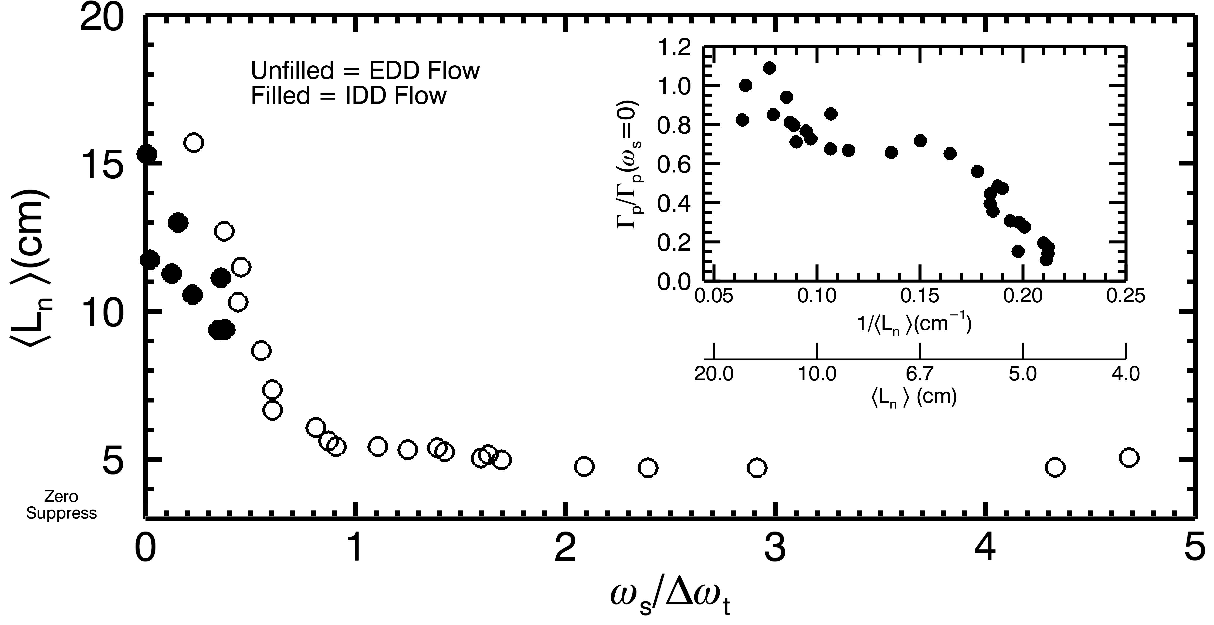
\includegraphics[width=8.5cm]{shearandgrad.pdf}% Here is how to import EPS art
\caption{\label{fig:shearandgrad} Gradient scale length versus shearing rate. Inset shows correlation of gradient scale length and turbulent particle flux. Note how this data is inconsistant with a Fick's Law like diffusion, which would be identified by a linearly increasing flux with gradient.}
\end{center}
\end{figure}

with average gradient scale length compared to the ratio of shearing rate to decorrelation rate. Both IDD and EDD flow and flow shear points lie on the same curve. Thus, confinement is insenstive to flow/flow-shear direction.

The change in confinement can be connected to a change in the turbulence properties of the plasma which dictate the turbulent flux. An overview of fluctuation power in saturated current (as a proxy for density) can be seen in Fig.~\ref{fig:powercontour} where the power as a function of frequency

\begin{figure}
\begin{center}
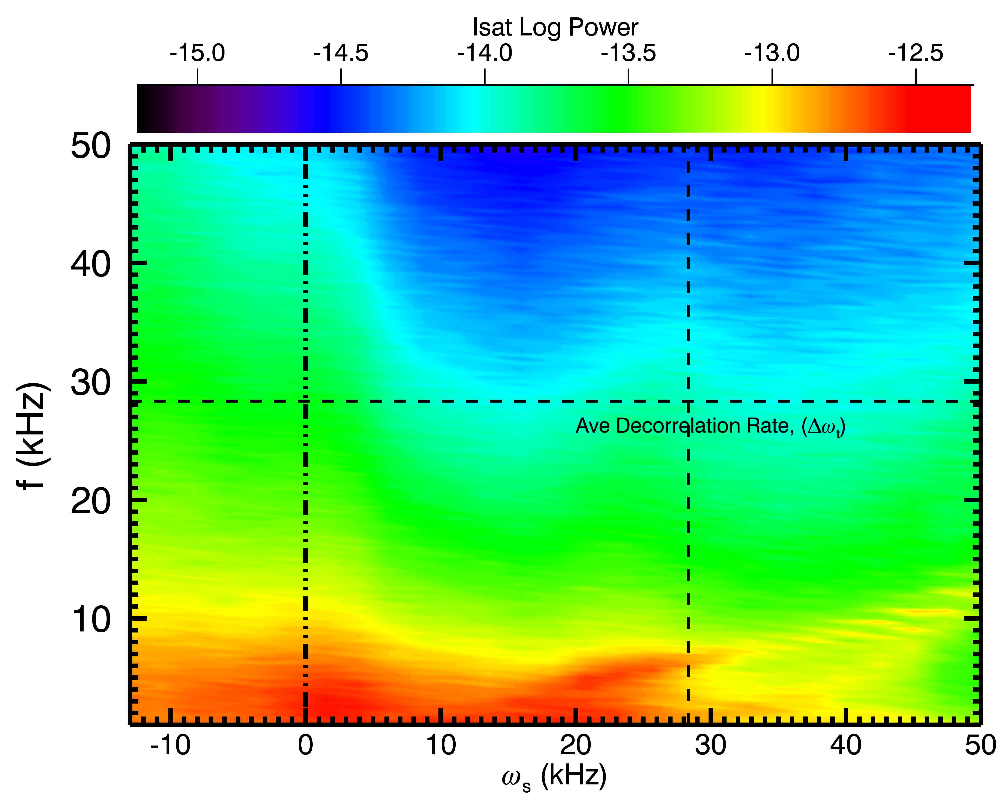
\includegraphics[width=8.5cm]{powercontour.pdf}% Here is how to import EPS art\
\caption{\label{fig:powercontour} Contour plot of log isat fluctuation power versus shearing rate and frequency. Dashed lines show location of decorrelation rate.}
\end{center}
\end{figure}

has been scaled to the turbulent decorrelation rate. The contour plot shows that most of the turbulent power is less than 10kHz and that in this range, power decreases overall with increasing shearing rate. A decrease by an order of magnitude of power occurs when the shearing rate reaches the decorrelation rate and further decreases at higher shearing. A coherent mode emerges at a frequency of about 8kHz about when the shearing rate is half the decorrelation rate. This mode increases in frequency linearly with shearing until it tapers out at about 12kHz at a shearing twice the decorrelation rate. The nature of this mode is still under investigation as well as its effects, if any, on the particle transport. 

The changes in gradient scale length and turbulence are indicative of an overall change in particle flux. This flux can be directly measured by correlating fluctuating isat with fluctuating radial flow---$E \times B$ flow using an electric field derived from two floating potential tips on either side of the isat measuring tip and rewritten in terms of the integral in \eqref{eq:fluxint}. Like gradient scale length, normalized average particle flux decreases with shearing rate scaled to the turbulent decorrelation rate as in Fig.~\ref{fig:fluxvsshear}.

\begin{figure}
\begin{center}
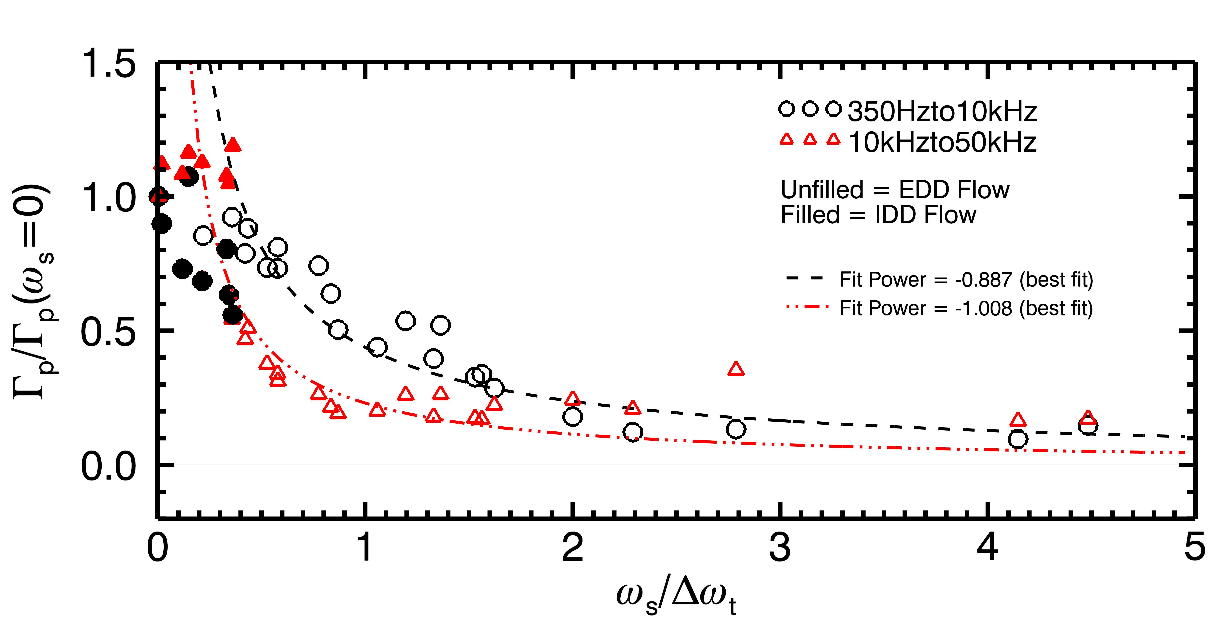
\includegraphics[width=8.5cm]{fluxvsshear.pdf}% Here is how to import EPS art
\caption{\label{fig:fluxvsshear} Particle flux as a function of shearing rate normalized to decorrelation rate. Black points show low frequency, red shows high. Filled symbols represent points with flow in IDD.}
\end{center}
\end{figure}

However, a clear difference emerges when the flux is bandwidth limited. The flux from 350Hz to 10kHz, where most of the fluctuation power is located, drops off gradually, hitting its minimum only at a shearing rate about three times the decorrelation rate. Higher bandwidth though, 10kHz to 50kHz, drops off faster, nearing its minimum when shearing equals decorrelation rate. Best fit lines from log-log plots of these scatters using a power law form of $\left(\omega_{s}/\Delta \omega_{t}\right)^{\alpha}$ yield exponents of $\alpha = -0.887$ for the low bandwidth flux and about $\alpha = -1.008$ for the high bandwidth flux. 

The reason for the difference becomes evident when the flux is examined by its separate components as in Fig.~\ref{fig:fluxcomps}.

\begin{figure}
\begin{center}
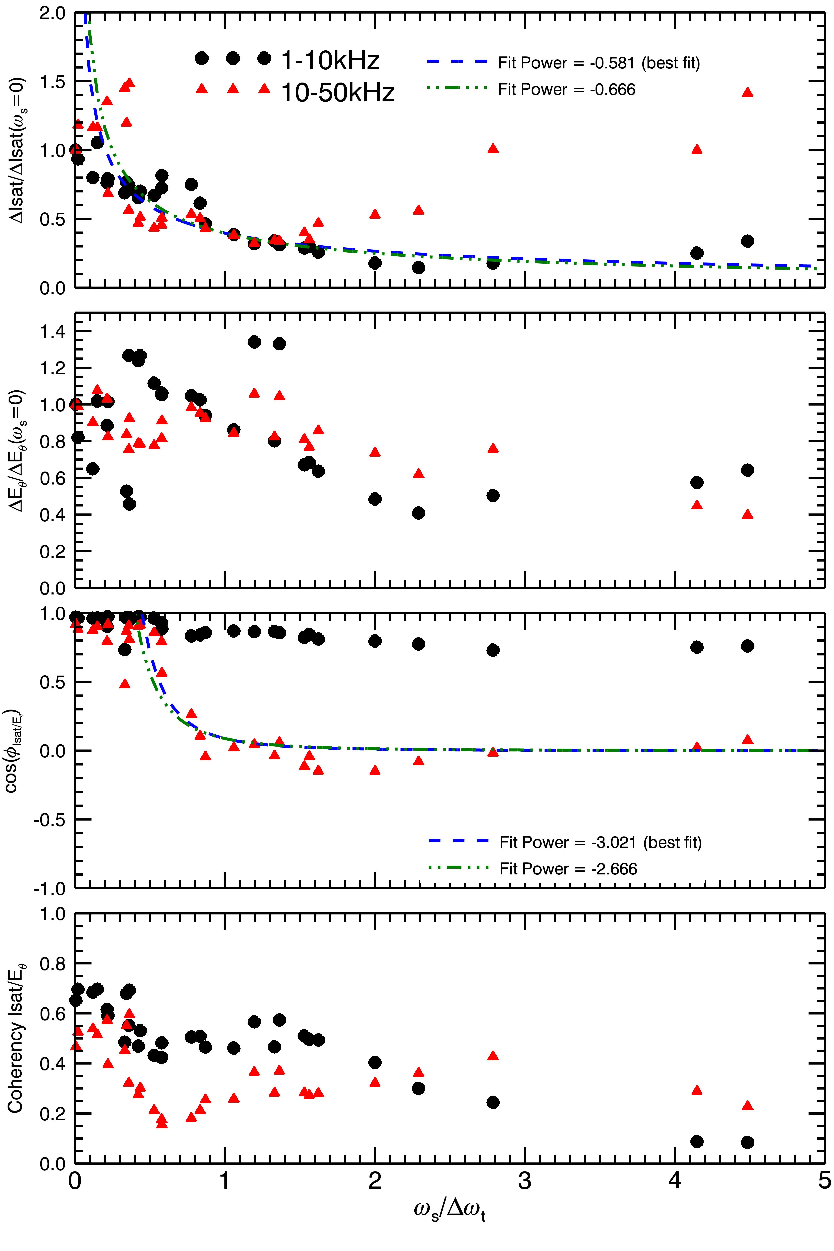
\includegraphics[width=8.5cm]{fluxcomps.pdf}% Here is how to import EPS art
\caption{\label{fig:fluxcomps} Components of particle flux versus shearing rate including isat/Density fluctuation power(a), electric field fluctuation power(b), crossphase(c) and coherency(d) with black points for low frequency, red for high.}
\end{center}
\end{figure}

The top two plots show fluctuation power---isat and electric field---as functions of normalized shearing rate, while the bottom two show crossphase and coherency respectively. For low bandwidth, isat power decreases gradually, with a power fit of $\alpha = 0.581$. Crossphase, on the other hand, does not decrease. In this bandwidth then, decreases in flux are primarily due to decreasing turbulent power. For high bandwidth flux, though, the opposite appears to be true. While isat fluctuations do decrease initially, they actually begin to increase at high shearing rates. In this case, the decrease in flux is primarily due to the drop in crossphase and to some extent coherency, regardless of growing turbulent power. A fit to this high frequency crossphase calculation yields $\alpha = -3.021$.  Electric field fluctuations, meanwhile, appear to be mostly unaffected by shearing. For both high and low frequency, the fluctuation power is reduced by no more than 50\% with even the highest shearing achieved. For comparison to BDT theory, a curve of power $\alpha = -(2/3)$ is plotted for isat fluctuations, while a curve of power $\alpha = -(8/3)$, two powers larger than $-(2/3)$, is show for the crossphase plot.

Using a cross-correlation technique, we can show the modifications of turbulent structures by azimuthal shearing, specifically the shortening of the radial correlation length Fig.~\ref{fig:radcorr}.

\begin{figure}
\begin{center}
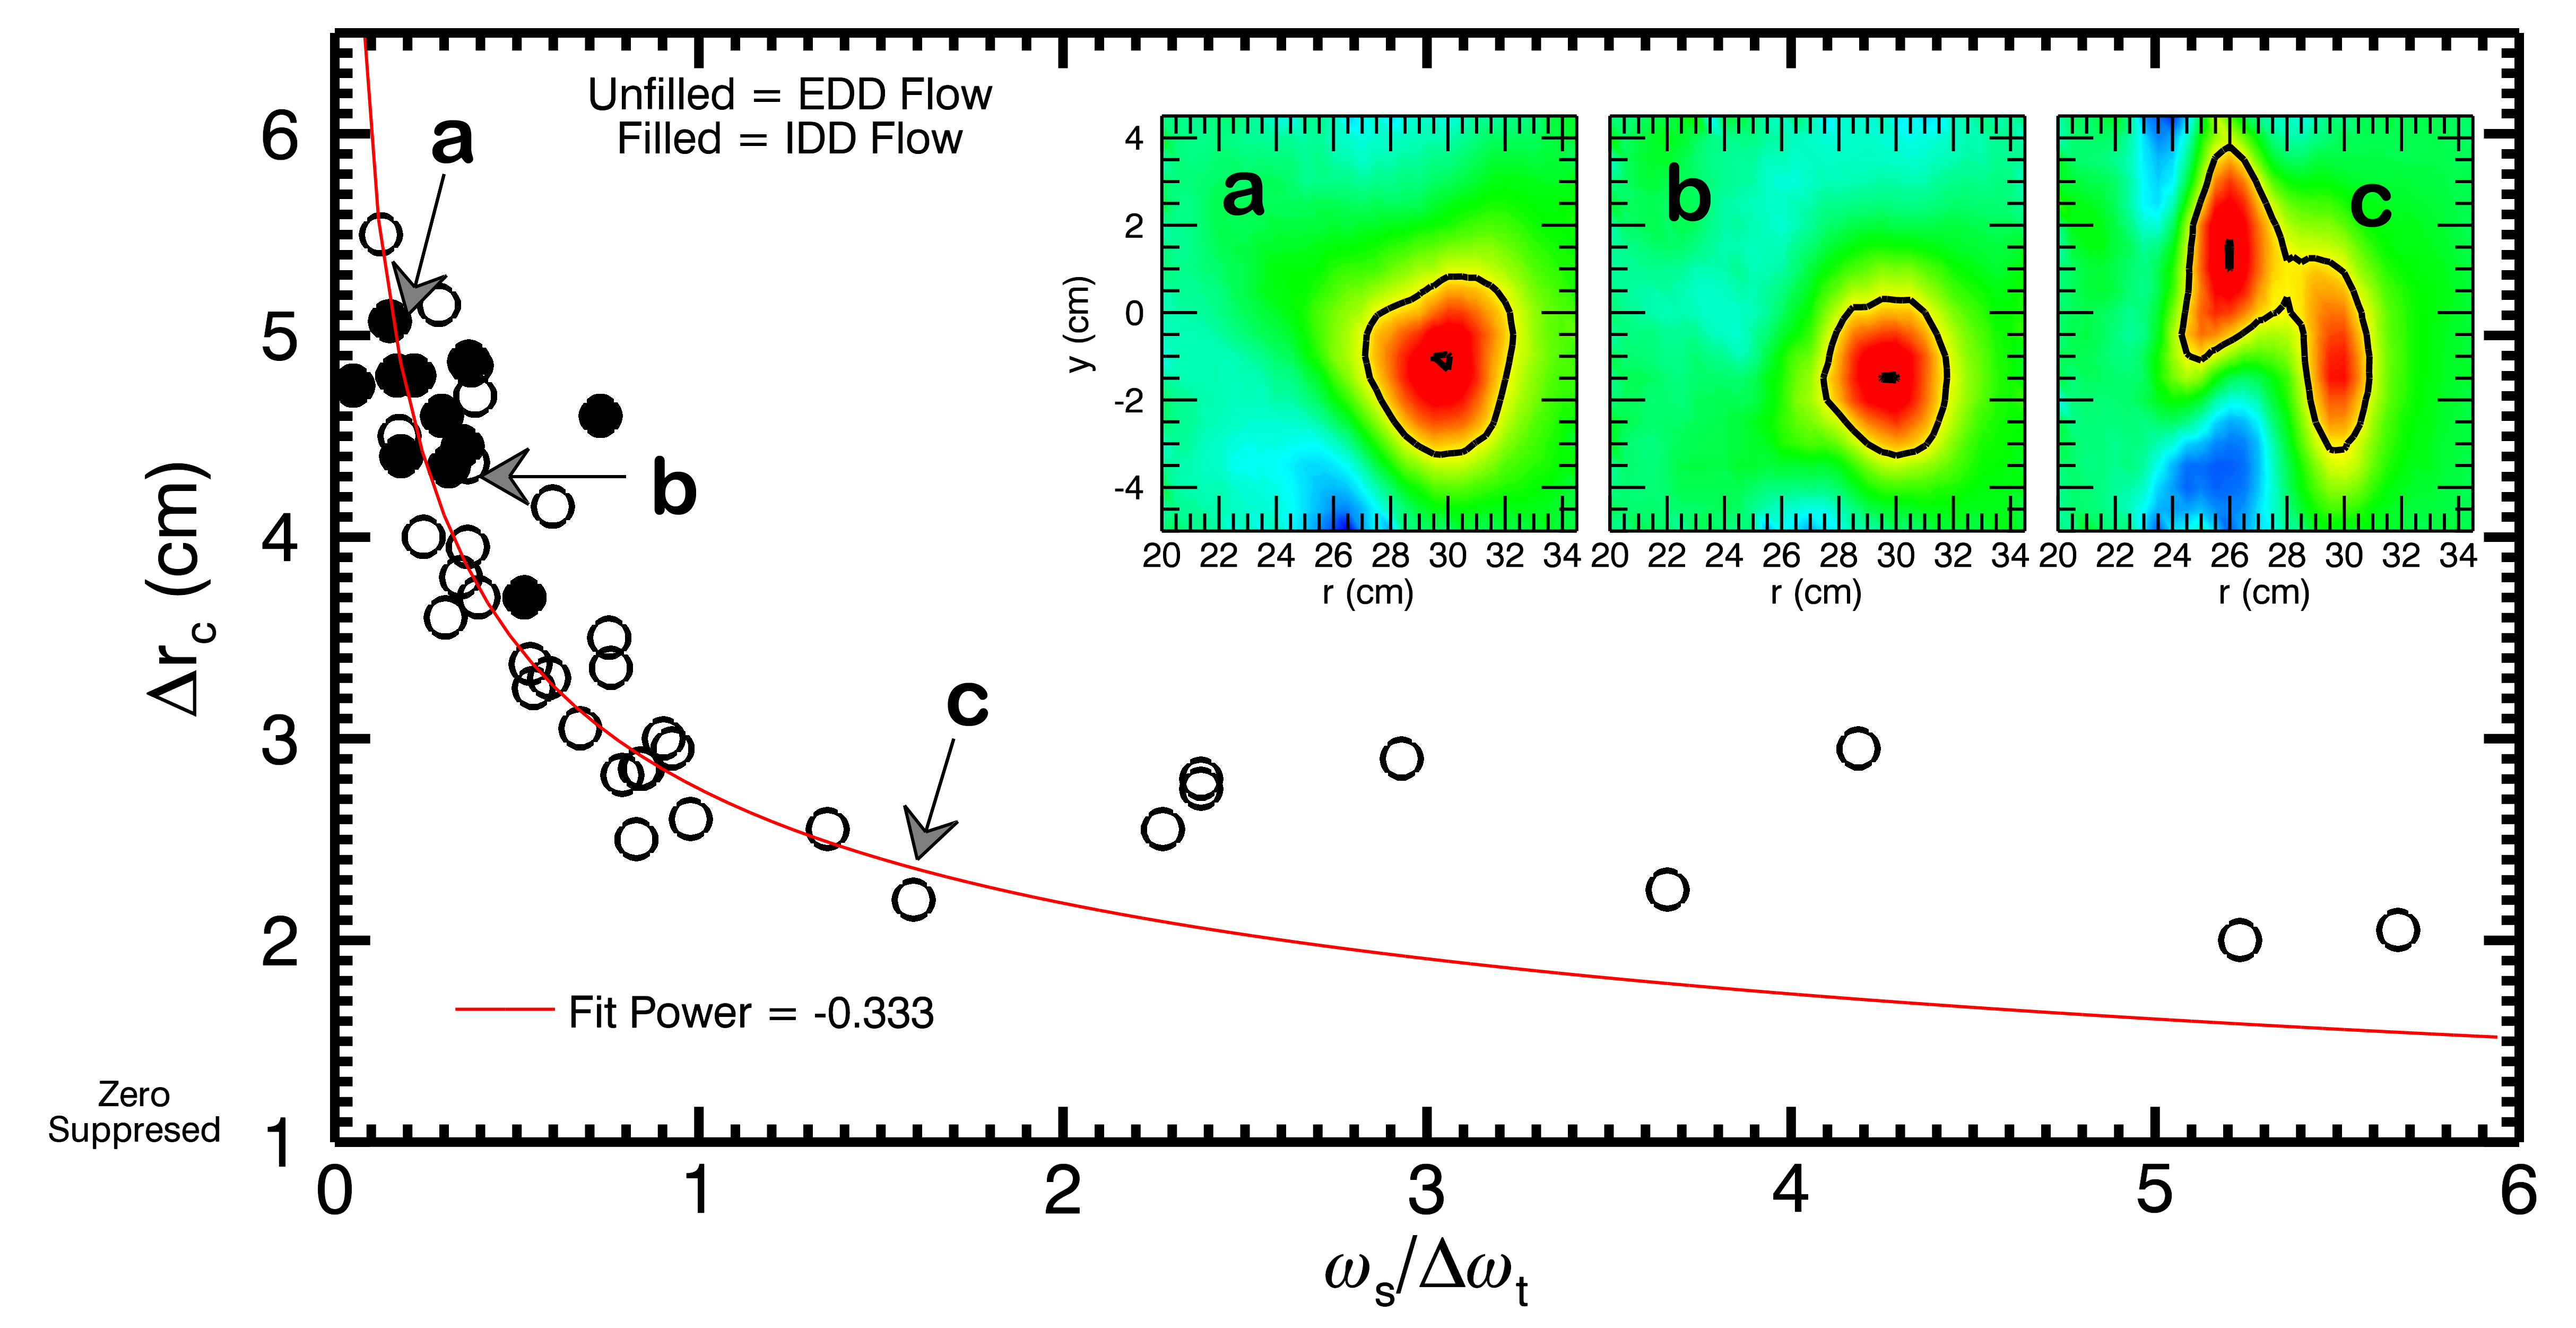
\includegraphics[width=8.5cm]{radcorr.pdf}% Here is how to import EPS art
\caption{\label{fig:radcorr} Measured radially correlation length with reference probes at 28,29,30,31 or 32cm and shows a decrease with flux that can be nearly fit to a power-law of -1/3. Inset shows 2D correlation length with reference probe at 30cm in azimuthal plane for low IDD flow shearing, no shear and high EDD flow shearing. The decrease in radial correlation can be seen as well as slight tilting depending on the direction of shear. A mode appears at higher shearings which appears to slightly extend correlation length.}
\end{center}
\end{figure}

The radially correlation length here is defined as the width of the contour plot to decrease to one-half its maximum value which occurs at the reference point, represented by the black curve in the inset of Fig.~\ref{fig:radcorr} and is normalized to the radial correlation length in the no-shear state. This correlation length decreases with shearing rate roughly following a power-law with $\alpha = -(1/3)$ indicating the sheared flow's ability to decrease the radial extend of a turbulent eddy. Like the flux and fluctuation data, the suppression begins with relatively little shearing. The correlation lengths can also be separated by frequency. High frequency correlation functions tend to be smaller than low frequency ones, though the normalized differences between the regimes is low. Note how IDD flow structures appear to grow someone wider with shear rather than EDD flow structures as show by the filled symbols. This may be due to contributions from a growing coherent mode with shear which is much more apparent and distinct in the EDD flow direction. This mode evidence in the correlation length can also be seen in the isat power spectrum beginning to grow in the regime of shearing where it is nearly equal to the decorrelation rate. This mode also appears to grow linearly in frequency with shearing rate. In is unclear what the orgin of this mode is---whether it is a drift-wave or flute-like Kelvin Helmholtz or rotational interchange---as well as what effect is has on the turbulence or flux. 

This letter presents the first detailed scan of shearing rate in a linear device and has shown a clear effect of particle flux and density confinement through both the mechanisms of turbulent fluctuation reduction and change in crossphase of saturated current and electric field. Moreover, the scan has allowed for comparison to theory predictions of the effect of shearing on both fluctuation power and crossphase. Fits of the data for both fluctuations and crossphase are consistent with the power law predictions proposed.

%\nocite{*}
\bibliography{FlowModPRL_bib}% Produces the bibliography via BibTeX.

\end{document}
%
% ****** End of file aipsamp.tex ******
